\DeclareOption*{\PassOptionsToClass{\CurrentOption}{abntex2}}
\ProcessOptions

\documentclass[
	% -- opções da classe memoir --
	12pt,				% tamanho da fonte
	openright,			% capítulos começam em pág ímpar (insere página vazia caso preciso)
	oneside,			% para impressão em verso e anverso. Oposto a oneside
	a4paper,			% tamanho do papel. 
	% -- opções da classe abntex2 --
	%chapter=TITLE,		% títulos de capítulos convertidos em letras maiúsculas
	%section=TITLE,		% títulos de seções convertidos em letras maiúsculas
	%subsection=TITLE,	% títulos de subseções convertidos em letras maiúsculas
	%subsubsection=TITLE,% títulos de subsubseções convertidos em letras maiúsculas
	% -- opções do pacote babel --
	english,			% idioma adicional para hifenização
	french,				% idioma adicional para hifenização
	spanish,			% idioma adicional para hifenização
	brazil				% o último idioma é o principal do documento
	]{abntex2}

\usepackage{setspace}
\usepackage{conf-ifsc}
\usepackage{hyperref}
\usepackage{graphicx}
\usepackage{caption}
\usepackage{subcaption}
\usepackage[utf8]{inputenc}
\usepackage{listings}
\usepackage{xcolor}
\usepackage{trivfloat}
\trivfloat{quadro}
\usepackage{enumitem}
\usepackage{xcolor}
\usepackage{multicol}
\usepackage{multirow}
\usepackage{hyperref}
\usepackage{float}
\floatstyle{plaintop}
\restylefloat{quadro}
\usepackage{chngcntr}
\usepackage{lipsum}
\usepackage{tocloft}
\usepackage{tocvsec2}
\usepackage{boxhandler}
\usepackage[font={bf,small},labelfont=small]{caption}


\newcommand{\source}[1]{\caption*{\normalfont Fonte: {#1}}}


\counterwithout{equation}{chapter}
\counterwithout{figure}{chapter}
\counterwithout{table}{chapter}

\newcommand\ChangeRT[1]{\noalign{\hrule height #1}}


\definecolor{codegreen}{rgb}{0,0.6,0}
\definecolor{codegray}{rgb}{0.5,0.5,0.5}
\definecolor{codepurple}{rgb}{0.58,0,0.82}
\definecolor{backcolour}{rgb}{0.95,0.95,0.92}

\lstdefinestyle{mystyle}{
    backgroundcolor=\color{backcolour},   
    commentstyle=\color{codegreen},
    keywordstyle=\color{magenta},
    numberstyle=\tiny\color{codegray},
    stringstyle=\color{codepurple},
    basicstyle=\ttfamily\footnotesize,
    breakatwhitespace=false,         
    breaklines=true,                 
    captionpos=b,                    
    keepspaces=true,                 
    numbers=left,                    
    numbersep=5pt,                  
    showspaces=false,                
    showstringspaces=false,
    showtabs=false,                  
    tabsize=2
}

\lstset{style=mystyle}

%---------------------------------------------------------------------%
%---------------------------------------------------------------------%
% Informações de dados para CAPA e FOLHA DE ROSTO
%---------------------------------------------------------------------%
%---------------------------------------------------------------------%

\titulo{SISTEMAS V2X E A EVOLUÇÃO DA CONECTIVIDADE VEICULAR: Análise da evolução tecnológica e simulação de benefícios}

\autor{VINICIOS DE AZEVEDO KRAUS}

\local{JOINVILLE}

\data{2026}

\orientador[Orientador:\\]{Stefano Romeu Zeplin, Mestre}


%\coorientador[Coorientador:\\]{Nome do coorientador}

\tipotrabalho{Monografia (Graduação)}

% O preambulo deve conter o tipo do trabalho, o objetivo, o nome da instituição e a área de concentração 
\preambulo{Trabalho de Conclusão de Curso submetido ao Instituto Federal de Educação, Ciência e Tecnologia de Santa Catarina como parte dos requisitos para obtenção do título de Engenheiro Eletricista.}

% \textoaprovacao{Este Trabalho foi julgado adequado para obtenção do Título de Engenheira Eletrônica em abril de 2021 e aprovado na sua forma final pela banca examinadora do Curso de Engenharia Eletrônica do instituto Federal de Educação Ciência, e Tecnologia de Santa Catarina.}



%---------------------------------------------------------------------%
% Início do documento
%---------------------------------------------------------------------%

\begin{document}



\selectlanguage{brazil}
\frenchspacing 


% ----------------------------------------------------------
% ELEMENTOS PRÉ-TEXTUAIS
% ----------------------------------------------------------
% \pretextual

\imprimircapa
\imprimirfolhaderosto* %(o * indica que haverá a ficha bibliográfica)

%---------------------------------------------------------------------%
% ATENÇÃO - Pergunte para a Biblioteca do IFSC
% Inserir a ficha bibliografica - 
%
% Para gerar a ficha catalográfica acesse:
% http://ficha.florianopolis.ifsc.edu.br/
% Precisa ser feito pelo navegador Mozilla Firefox
%---------------------------------------------------------------------%

%\imprimirficha{pdf/fichacatalografica.pdf}
%\cleardoublepage

%---------------------------------------------------------------------%
% Inserir folha de aprovação
%---------------------------------------------------------------------%


%\imprimiraprovacao
%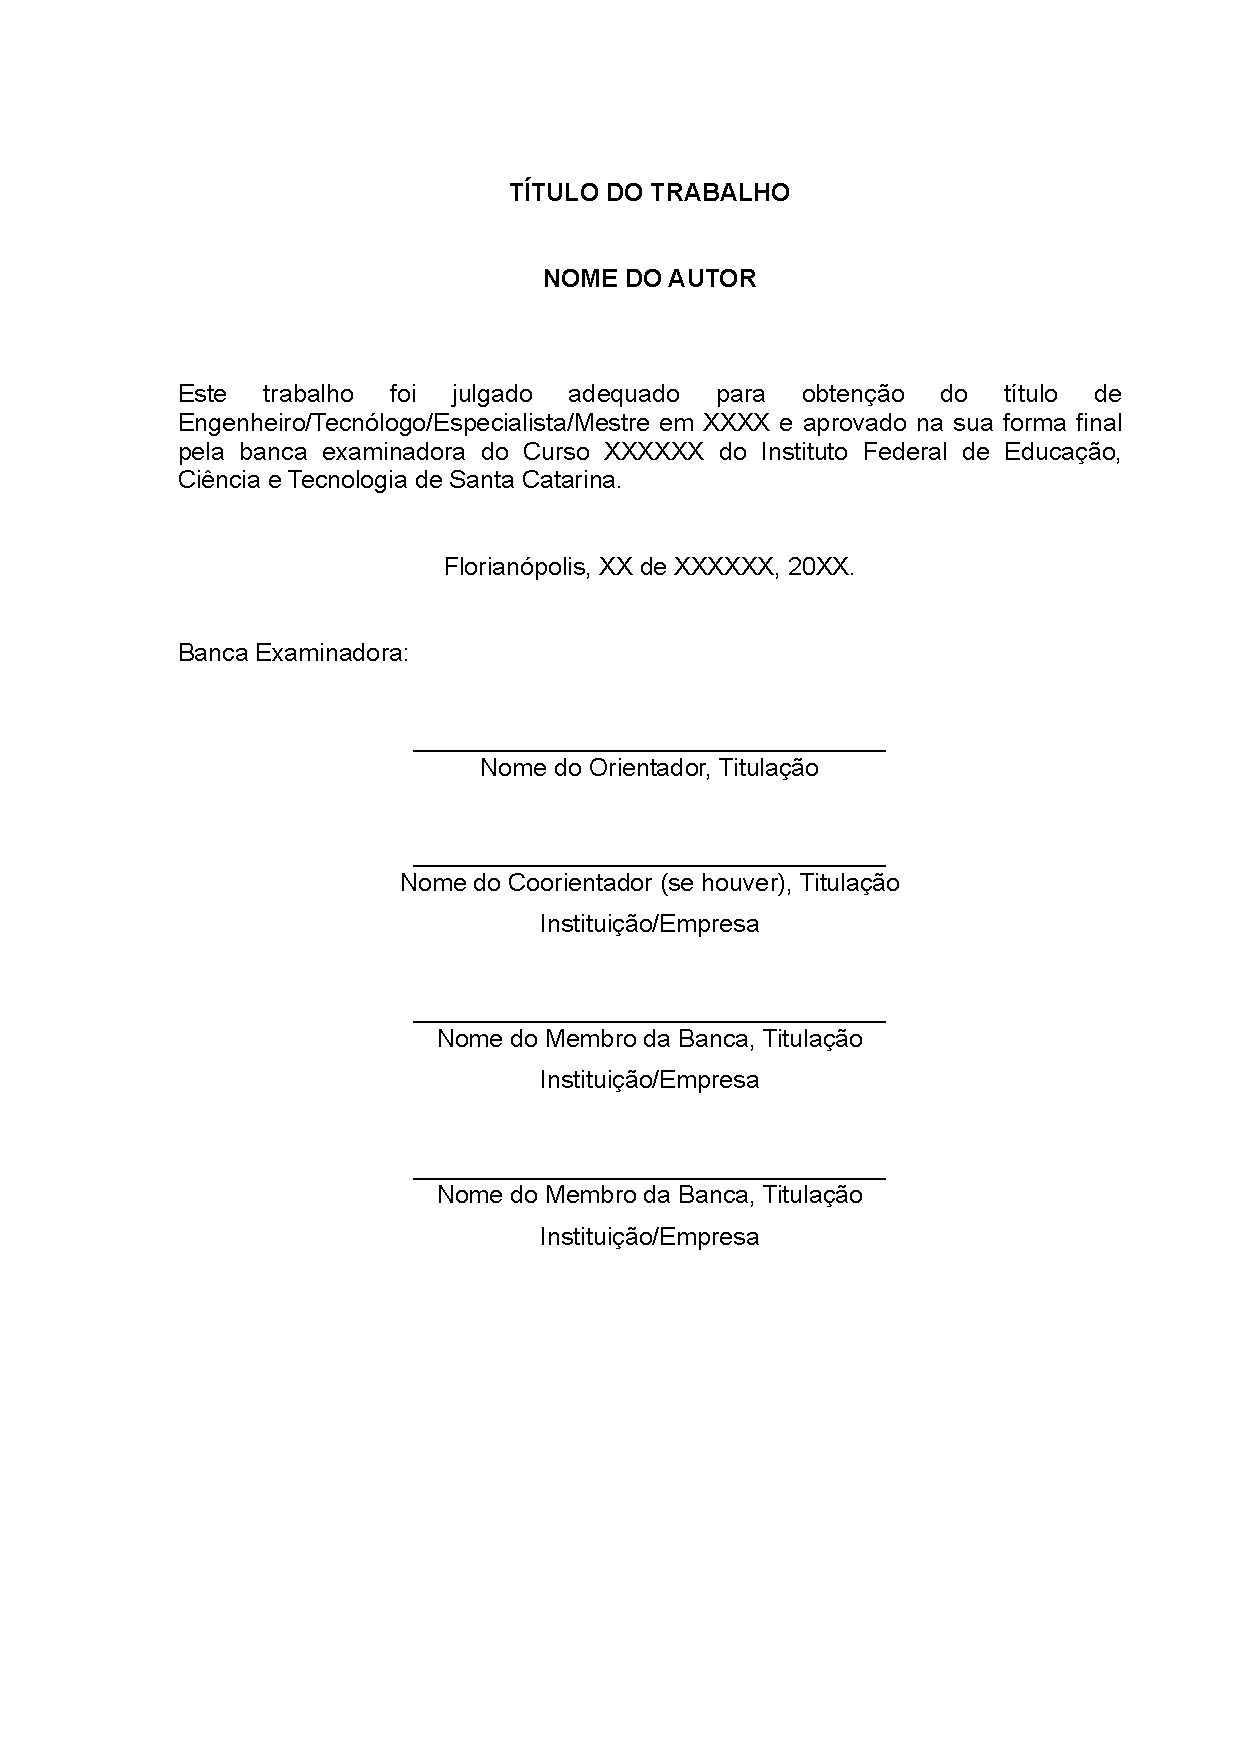
\includepdf[pages=-]{pdf/tcc-aprovado.pdf}

%\cleardoublepage

%---------------------------------------------------------------------%
% Dedicatória
%---------------------------------------------------------------------%
\begin{dedicatoria}
    \vspace*{\fill}
	\begin{flushright}
    		(Dedicatória é um elemento opcional.\\ 
            Texto alinhado no canto inferior direito.\\
            Não deve ultrapassar uma página.)
	\end{flushright}
\end{dedicatoria}




%---------------------------------------------------------------------%
% Agradecimentos
%---------------------------------------------------------------------%
\begin{agradecimentos}
    Elemento opcional que não pode ultrapassar o limite de uma página.
\end{agradecimentos}
% ---

%---------------------------------------------------------------------%
% Epígrafe
%---------------------------------------------------------------------%
\begin{epigrafe}
    \vspace*{\fill}
	\begin{flushright}
    		(Epígrafe é um elemento opcional.\\
    		Texto alinhado no canto inferior direito.\\
            Não deve ultrapassar uma página.)
	\end{flushright}
\end{epigrafe}

%---------------------------------------------------------------------%
% RESUMOS
%---------------------------------------------------------------------%
% resumo em português
\setlength{\absparsep}{18pt} % ajusta o espaçamento dos parágrafos do resumo
\renewcommand{\baselinestretch}{1} 
\begin{resumo}
    %O resumo deve mostrar a natureza e o objetivo do trabalho, o método que foi empregado, os resultados e as conclusões. O resumo deve conter entre 150 e 500 palavras e constitui-se de um único parágrafo, sem recuo.

    Este trabalho analisa a trajetoria da telematica veicular e a evolução dos sistemas V2X (Vehicle-to-Everything), analisando a transição de tecnologias que
    no passado focavam em um monitoramento isolado de veículos para uma abordagem mais integrada e conectada, onde os veículos se comunicam entre si e com as
    infraestruturas ao redor, num Sistema de Transporte Inteligente Cooperativo (C-ITS). A pesquisa destaca a evolução dos padrões de conectividade veicular,
    desde os primeiros sistemas de monitoramento de frotas, passando por tecnologias como DSRC (Dedicated Short-Range Communications) no padrão IEEE 802.11p,
    até a adoção de tecnologias celulares como C-V2X (Cellular Vehicle-to-Everything) usando da conectividade 4G e 5G. A pesquisa realizada se fundamenta no
    desenvolvimento de uma simulação de tráfego utilizando o SUMO (Simulation of Urban Mobility) integrado com o OMNeT++ e o framework Veins para avaliar os
    benefícios dos sistemas V2X em cenários urbanos. O propósito é demonstrar através de simulações e da base teórica, como a evolução dos sistemas V2X tem o
    potencial de melhorar a segurança viária, mitigando conflitos e optimizando o fluxo de tráfego.
    
    Os resultado da análise indicam que (completar com o que for encontrado na analise)...



 
   \noindent 
    \textbf{Palavras-chave}: V2X. C-V2X. Simulação de tráfego. Segurança e eficiência viária.
\end{resumo}

% resumo em inglês
\renewcommand{\baselinestretch}{1} 
\begin{resumo}[Abstract]
 \begin{otherlanguage*}{english}

   This work analyzes the trajectory of vehicular telematics and the evolution of V2X (Vehicle-to-Everything) systems, examining the transition from technologies
   that in the past focused on isolated vehicle monitoring to a more integrated and connected approach, where vehicles communicate with each other and with
   surrounding infrastructures in a Cooperative Intelligent Transport System (C-ITS). The research highlights the evolution of vehicular connectivity standards,
   from early fleet monitoring systems, through technologies such as DSRC (Dedicated Short-Range Communications) under the IEEE 802.11p standard, to the adoption
   of cellular technologies such as C-V2X (Cellular Vehicle-to-Everything) using 4G and 5G connectivity. The research is based on the development of a traffic
   simulation using SUMO (Simulation of Urban Mobility) integrated with OMNeT++ and the Veins framework to evaluate the benefits of V2X systems in urban
   scenarios. The purpose is to demonstrate through simulations and the theoretical basis how the evolution of V2X systems has the potential to improve road
   safety, mitigating conflicts and optimizing traffic flow.
   
   The results of the analysis indicate that (to be completed with the findings from the analysis)...

   %\vspace{-0.8cm}
 
   \noindent 
   \textbf{Keywords}: V2X. C-V2X. Traffic simulation. Road safety and efficiency.
 \end{otherlanguage*}
\end{resumo}


%---------------------------------------------------------------------%
% inserir lista de ilustrações
%---------------------------------------------------------------------%
\renewcommand{\listfigurename}{Lista de Figuras}
\pdfbookmark[0]{\listfigurename}{lof}
\listoffigures*
\cleardoublepage

%---------------------------------------------------------------------%
% inserir lista de quadros
%---------------------------------------------------------------------%

\renewcommand{\listquadroname}{Lista de quadros}
\newfloat{quadro}{\quadroname}{loq}[chapter]
\setfloatlocations{quadro}{hbtp}
\newlistof{listofquadros}{loq}{\listquadroname}
\newlistentry{quadro}{loq}{0}
\renewcommand{\cftquadroname}{\quadroname\space}
\renewcommand*{\cftquadroaftersnum}{\hfill\textendash\hfill}
\counterwithout{quadro}{chapter}
\listofquadros* 
\cleardoublepage



%---------------------------------------------------------------------%
% inserir lista de tabelas
%---------------------------------------------------------------------%
\pdfbookmark[0]{\listtablename}{lot}
\listoftables*
\cleardoublepage

%---------------------------------------------------------------------%
% inserir lista de listings
%---------------------------------------------------------------------%
%\pdfbookmark[0]{\lstlistlistingname}{lol}
%\listoflistings
%\cleardoublepage

%---------------------------------------------------------------------%
% inserir lista de abreviaturas e simbolos
%---------------------------------------------------------------------%
%\listofabrev{tex/00-Abreviaturas}
\imprimirlistadeabreviaturas

% \imprimirlistadesimbolos
\cleardoublepage

%---------------------------------------------------------------------%
% inserir o sumario

%---------------------------------------------------------------------%


\setlength{\cftbeforechapterskip}{4pt plus 0pt}
\pdfbookmark[0]{\contentsname}{toc}


\tableofcontents*


\cleardoublepage

% ----------------------------------------------------------
% ELEMENTOS TEXTUAIS
% ----------------------------------------------------------
\textual

% ----------------------------------------------------------
% Inclusão dos capítulos que estão em outros arquivos .tex
% ----------------------------------------------------------

\chapter{Introdução}

Desde que o primeiro veículo a combustão interna foi produzido lá no final do século XIX por Karl Benz, a ideia geral de automóvel não sofreu grandes alterações,
mantendo uma essencia quase completamente mecânica por mais de um século, usando o motor a combustão para propulção e as rodas e eixos para transmissão de potência
para o solo. Mas como destaca Hodel \cite{ref:hodel}, o que mais mudou nessas ultimas décadas foi o desenvolvimento de sistemas eletrônicos embarcados nos veículos,
saindo de um produto puramente mecânico para um produto que cada vez mais intregra sistemas computacionais e softwares.

Essa revolução tecnológica vem após a introdução das Unidades de Controle Eletrônico (ECUs) nos veículos. Conforme destaca Jubelli \cite{ref:jubelli}, tudo se
iniciou por volta de 1970 e evoluiu para os atuais sistemas de controle eletrônicos embarcados, onde cada carro pode possuir mais de 80 ECUs, responsáveis por
controlar e monitorar uma variedade de funções do automóvel, gerenciando sistema criticos como o motor, transmissão e segurança. O aumento exponencial da
complexidade empregada nesses sistemas impulsionou o surgimento de Sistemas de Transporte Inteligente (ITS), que buscam integrar comunicação e controle para
melhorar a segurança, eficiência e sustentabilidade do transporte.

Como parte da evolução dos ITS, hoje já falamos em Sistemas de Transporte Inteligente Cooperativo (C-ITS), onde a conciência cooperativa é concebida através da
tecnologia V2X (\textit{Vehicle-to-Everything}). Automóveis convencionais geralmente possuem sensores como radares e câmeras para monitorar o ambiente ao redor,
mas acabam sendo limitados pela linha de visão e alcance desses sensores. O V2X, por outro lado, permite trazer uma visão além da linha de visão do próprio veículo,
possibilitando a comunicação entre outros veículos, infraestrutura rodoviária e até mesmo pedestres, criando uma maior conciência sobre o ambiente próximo. Essa
comunicação cooperativa foi viabilizada pelas tecnologias DSRC ou C-V2X, que funcionam respectivamente pelos padrões da IEEE 802.11p e por redes celulares LTE e 5G,
permitindo a troca de informações em tempo real entre os participantes do sistema de transporte.

\abreviatura{C-ITS}{Sistema de Transporte Inteligente Cooperativo}
\abreviatura{DSRC}{\textit{Dedicated Short-Range Communications}}
\abreviatura{C-V2X}{\textit{Cellular Vehicle-to-Everything}}
\abreviatura{SUMO}{\textit{Simulation of Urban Mobility}}


\section{Justificativa}

Texto texto texto texto texto texto texto texto texto texto texto texto texto texto texto texto texto texto texto texto texto texto texto texto texto texto texto texto texto texto texto texto texto texto texto texto texto texto texto.

\section{Definição do Problema}

Texto texto texto texto texto texto texto texto texto texto texto texto texto texto texto texto texto texto texto texto texto texto texto texto texto texto texto texto texto texto texto texto texto texto texto texto texto texto texto \cite{ref:hodel}.

\section{Objetivo Geral}

Texto texto texto texto texto texto texto texto texto texto texto texto texto texto texto texto texto texto texto texto texto texto texto texto texto texto texto texto texto texto texto texto texto texto texto texto texto texto texto.

\section{Objetivos Específicos}

Texto texto texto texto:
\begin{alineas}
    \item texto texto texto texto texto texto texto texto texto texto texto texto texto texto texto texto texto texto texto texto texto texto texto texto texto texto texto texto texto texto texto texto texto texto texto texto texto texto;
    \item texto texto texto texto texto texto texto texto texto texto texto texto texto texto texto texto texto texto texto texto texto texto texto texto texto texto texto texto texto texto texto texto texto texto texto texto texto texto; 
    \item texto texto texto texto texto texto texto texto texto texto texto texto texto texto texto texto texto texto texto texto texto texto texto texto texto texto texto texto texto texto texto texto texto texto texto texto texto texto.
\end{alineas}
    
\section{Estrutura do Trabalho}

Texto texto texto texto texto texto texto texto texto texto texto texto texto texto texto texto texto texto texto texto texto texto. 

\chapter{Fundamentação Teórica}

O capítulo atual traz a fundamentação teórica necessária para o desenvolvimento deste trabalho, abrangendo a evolução da eletrônica e sistemas
embarcados veiculares, e a tecnologia de comunicação veículo-a-tudo (V2X). Serão introduzidos conceitos, definições e padrões tecnológicos, visando
construir uma base teórica sólida para desenvolver a simulação de tráfego e a subsequente análise dos benefícios da conectividade cooperativa na
segurança e eficiência do trafego urbano.

\section{Fundamentos da Eletrônica Veicular}

O mercado automotivo global na atualidade apresenta grande parte da competitividade e diferenciação entre os fabricantes quando o assunto é a eletrônica
integrada nos veículos. Um estudo publicado por \cite{ref:bccresearch} realizou a análise da cadeia de suprimentos e levantou dados sobre o crescimento
do mercado de eletrônicos na industria automotiva, onde os componentes eletrônicos já representam cerca de 30\% do valor valor total de fabricação de um
novo veículo movido a motores de combustão interna. Com a consolidação de novas tecnologias de conectividade, direção autônoma e eletrificação, projeta-se
que a eletrônica atinja uma participação de 50\% do valor total de fabricação de um veículo a combustão e chegando a 70\% em veículos elétricos (EVs).

Essa infraestrutura tecnológica é bem mais visível em veículos premium, que conseguem integrar mais de 100 ECUs interconectadas e distribuidas por todo o
veículo. Diversas redes diferentes como CAN, LIN, FlexRay e Ethernet são utilizadas para conectar os diversos subsistemas, assim como é mostrado na
Figura \ref{fig:vehicle_electronics_network}, onde múltiplas ECUs, sensores e atuadores se comunicam por meio de barramentos e redes de comunicação internas
ao veículo \cite{ref:leen2002}.

\begin{figure}[H]
    \centering
    \caption{Arquitetura típica de rede eletrônica veicular}
    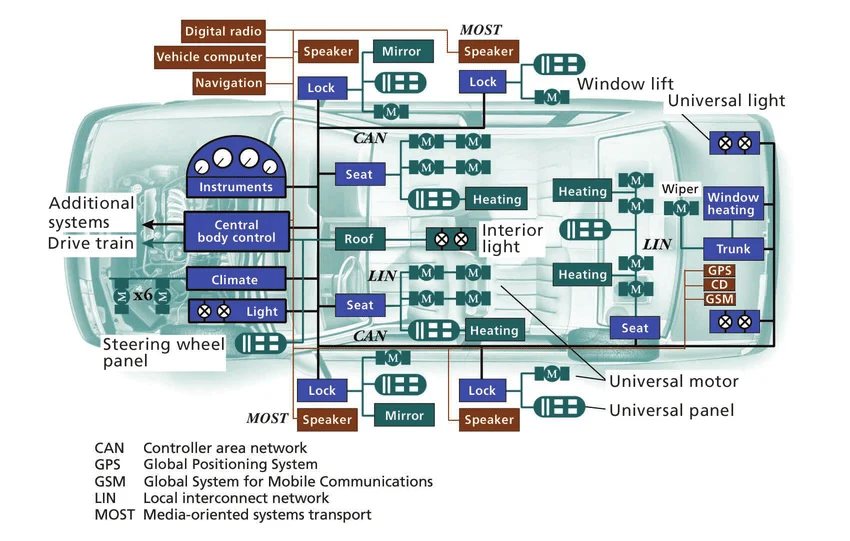
\includegraphics[width=0.85\linewidth]{figuras/vehicle_electronics_network.png}
    \label{fig:vehicle_electronics_network}
    \par\smallskip
    \small Fonte: Adaptado de Leen e Heffernan (2002).
\end{figure}

A Unidade de Controle Eletrônico (ECU) é o principal componente da arquitetura eletrônica moderna, operando de maneira dedicada funções específicas do
veículo. Tecnicalmente, as ECUs funcionam sob o modelo IPO (\textit{Input-Process-Output}), onde circuitos de entrada recebem sinais de sensores (como
temperatura e velocidade), microcontroladores processam os dados e executam algoritmos para tomada de decisão, e circuitos de saída utilizam os resultados
para controlar atuadores (como injetores de combustível e freios). De acordo com \cite{ref:munir2018}, os automóveis modernos evoluiram integrando uma centena
de processadores, que operam sob protocolos de comunicação em redes de alta velocidade para coordenar as funções do automóvel.

A integração dessas unidades de controle em uma arquitetura de rede complexa exige que o veículo seja tratado como um conjunto de sistemas distribuídos.
Funções criticas, como segurança ativa e controle de propulsão, dependem da comunicação eficiente entre varias ECUs através das redes do automóvel. Essa
grande quantidade de eletrônica integrada e uma crescente interdependência entre os subsistemas tornam o desenvolvimento, teste e validação de software
automotivo cada vez mais desafiadores, mas também traz a oportunidade do desenvolvimento de novas tecnologias e funcionalidades que permitem uma maior
consciência sobre o ambiente para uma melhor experiência de condução e segurança.

\section{Evolução da Eletrônica e Sistemas Embarcados}

A indústria automotiva tem passado por uma transformação significativa nas últimas décadas, tornando-se significativamente mais intensiva em sistemas
computacionais e softwares do que em sistemas mecânicos. Enquanto historicamente o desenvolvimento era dominado pela engenharia mecânica, hoje a parte
eletrônica e de software se tornaram o principal motor de inovação no setor automotivo. Essa transformação se iniciou por volta de 1970, com a introdução
das ECUs, que alterou as lógicas de comando das funcionalidades veículares.  

Veículos mais modernos apresentam um sistemas embarcados cada vez mais complexos, integrando uma variedade de radares, sensores e câmeras para aquisição de
dados. Como ilustrado na Figura \ref{fig:audi_a8}, o Audi A8 integra diversos componentes eletrônicos, que trabalham de forma conjunta, oferecendo ao motorista
funções avançadas de assistência à condução e segurança. Essa diversidade de dispositivos demonstra que a eletrônica se tornou algo fundamental para os veículos
atuais, trazendo tecnologias inovadoras ao mercado, como o sistema de direção autônoma e a conectividade veicular (V2X), que serão abordados posteriormente 
neste capítulo.

\begin{figure}[H]
    \centering
    \caption{Sensores e Câmeras do Audi A8}
    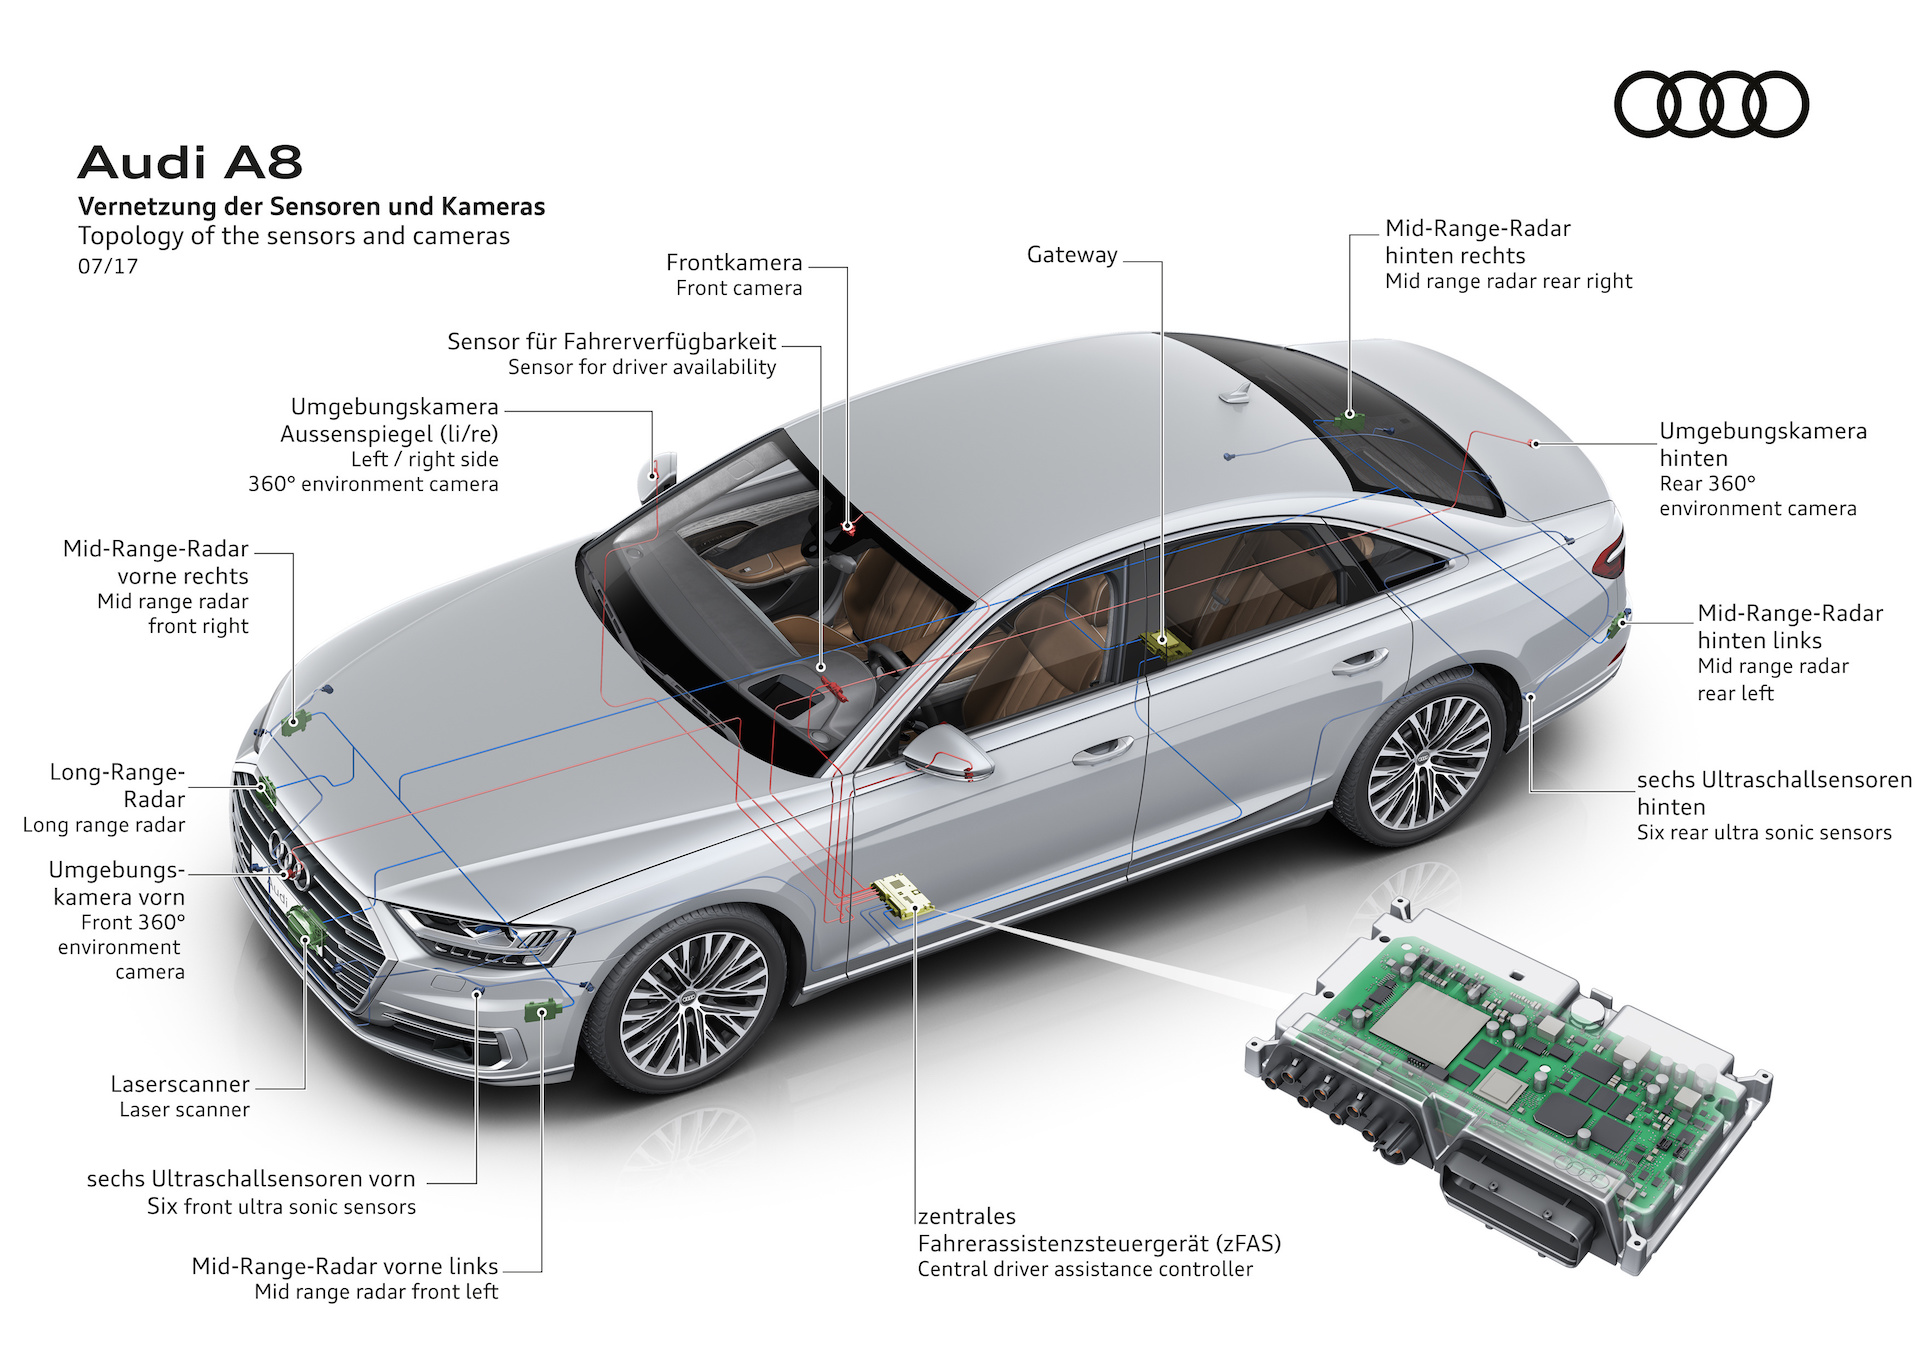
\includegraphics[width=0.85\linewidth]{figuras/audi_A8_sensors_and_cameras.jpg}
    \label{fig:audi_a8}
    \par\smallskip
    \small Fonte: Audi (2019).
\end{figure}

Como mencionado por \cite{ref:hodel} em seu trabalho sobre testes para software em sistemas embarcados automotivos, o setor está sendo impulsionado por
tecnologias como a eletrificação, a Internet das Coisas (IoT) e a automação, que além de necessitarem uma integração entre os subsistemas internos do veículo,
também necessitam uma comunicação com infraestruturas externas. Como esse nível de integração, fundamentamos a transição para um Sistema de Transporte Inteligente
(ITS), permitindo que o meio de transporte não sejam apenas limitados ao hardware instalado no veículo, mas também possam se comunicar com outros veículos e com
a infraestrutura urbana ao seu redor através da conectividade V2X.

\section{Tecnologia de Comunicação Veicular (V2X)}

A comunicação veicular consiste em uma tecnologia para troca de dados entre veículos e outros elementos do ambiente, aumentando a consciência situacional no
ambiente de tráfego, gestão operacional e a conveniência do usuário. A ideia principal desse tipo de comunicação é elevar o nível de segurança e eficiência do
transporte, permitindo que os automóveis recebam informações críticas que sistemas de bordo isolados não conseguem captar sozinhos, além de possibilitar
funcionalidades como a gestão de frotas em tempo real, monitoramento de condições de tráfego, atualizações de software \textit{over-the-air} (OTA) e serviços
de entretenimento conectados. Neste contexto, a literatura destaca que a comunicação \textit{Vehicle-to-Everything} (V2X) é projetada para ampliar o alcance
de detecção e percepção dos veículos além do que os sensores tradicionais locais podem alcançar \cite{ref:men2021}.

A implementação desse ecossistema tem como base dois padrões de comunicação principais: o DSRC (\textit{Dedicated Short Range Communications}) baseado no
padrão IEEE 802.11p, e o C-V2X (\textit{Cellular Vehicle-to-Everything}) desenvolvido pela 3GPP, que utiliza a infraestrutura de redes celulares para
comunicação. O DSRC foi o primeiro padrão a ser desenvolvido e testado, sendo utilizado principalmente para comunicação de curto alcance, enquanto o C-V2X é
uma tecnologia mais recente, que oferece maior alcance, capacidade de dados, maior confiabilidade e melhor desempenho em ambientes urbanos densos. Além disso,
o C-V2X é projetado para ser compatível com as futuras gerações de redes móveis, permitindo uma evolução contínua da tecnologia de comunicação veicular. 

\section{Modelagem e Simulação de Tráfego}

Texto texto texto texto texto texto texto texto texto texto texto texto texto texto texto texto texto texto texto texto texto texto texto texto texto texto texto texto texto texto texto texto texto. \cite{ref:mulligan}.


\subsubsection{Subtítulo Quaternário}

Texto texto texto texto texto texto texto texto texto texto texto texto texto texto texto texto texto texto texto texto texto texto texto texto texto texto texto texto texto texto texto texto texto  (conforme exposto na Figura \ref{fig:audi_a8}).

Texto texto texto texto texto texto texto texto texto texto texto texto texto texto texto conforme indica a Tabela \ref{tabela1}.

    

\begin{table}[h]
\centering
\caption{Produção de petróleo na Bahia}
\begin{tabular}{ c c }
\ChangeRT{2pt}
Ano  & Produção (1000 t) \\ \ChangeRT{2pt}
1996 & 2.536             \\ 
1997 & 2.665             \\ 
1998 & 3.056             \\ 
1999 & 3.567             \\ 
2021 & Atômica           \\ \ChangeRT{2pt}
\end{tabular}
\label{tabela1}
\\
\small{Fonte: Adaptado de ANP (2000).} 
\end{table}



    
    Texto texto texto texto texto texto texto texto texto texto texto texto texto texto texto texto texto texto texto texto texto texto texto texto texto texto texto texto texto texto texto texto texto 
    Texto texto texto texto texto texto texto texto texto texto texto texto texto texto texto texto texto texto texto texto texto texto texto texto texto texto texto texto texto texto texto texto texto como evidencia a Figura  \ref{fig:diagrama}.
    
\begin{quadro}[h]
\centering

\caption{Tipos de energia analisados}
\begin{tabular}{|c|c|}
\hline
\textbf{Ano} & \textbf{Tipos de energia} \\ \hline
2017         & Mecânica                  \\ \hline
2018         & Térmica                   \\ \hline
2019         & Elétrica                  \\ \hline
2020         & Química                   \\ \hline
2021         & Atômica                   \\ \hline
\end{tabular}
\label{quadro1}
\\
\small{Fonte: Elaboração própria (2021).} 
\end{quadro}
    
    
    \begin{figure}[H]
    	\centering
    	\caption{Diagrama Fasorial}
    	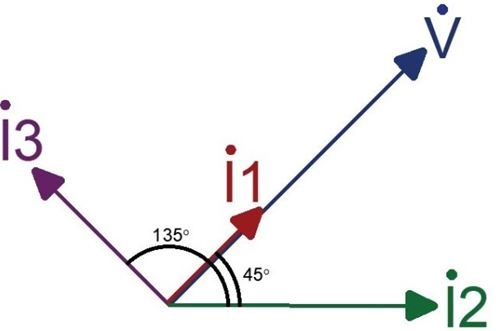
\includegraphics[scale=0.45]{figuras/diagrama.jpg}
    	\label{fig:diagrama}
    	\\
    	\vspace{0.2cm}\hspace{-3cm}\small{Fonte: Silva (2020).}
    \end{figure}
    
    Texto texto texto texto texto texto texto texto texto texto texto texto texto texto texto texto texto texto texto texto texto texto texto texto texto texto texto texto texto texto texto texto, conforme mostra a Equação \ref{eq:baskara}.
    
\begin{equation} \label{eq:baskara}
  x=\frac{-b\pm\sqrt{b^2-4ac}}{2a}
\end{equation} 

\chapter{Metodologia}

O presente capítulo descreve a metodologia empregada no desenvolvimento deste projeto, que se caracteriza pela união de diferentes áreas técnicas, como
a telecomunicação, sistemas embarcados, software/computação e tráfego urbano. A metodologia adotada é baseada em uma abordagem de pesquisa aplicada,
com foco na implementação prática por meio de simulações e validação dos conceitos estudados.

Um ponto crucial para o desenvolvimento deste trabalho é o uso de testes em ambiente virtual, que nos permite prever e analisar o comportamento do
sistema e encontrar possíveis falhas ou melhorias antes de uma implementação física. Validar virtualmente sistemas complexos é fundamental para
diminuir custos, otimizar recursos e limitar riscos, permitindo estudar cenários variados que podem ser encontrados no mundo real.

Para colocar esse estudo em prática, utiliza-se uma combinação de ferramentas de simulação, sendo o SUMO para modelagem de tráfego, o OMNeT++ para
simulação de redes e o Veins para integração entre ambos. A metodologia inclui a coleta de dados, modelagem do ambiente de tráfego, implementação
dos protocolos de comunicação V2X, execução das simulações e análise dos resultados obtidos.

\section{Análise do ambiente de tráfego}

\begin{alineas}
    \item Caracterização do ambiente de tráfego urbano;
    \item Requisitos de conectividade;
\end{alineas}

\section{Especificações da arquitetura C-V2X}
\begin{alineas}
    \item Padrões de comunicação;
    \item Mensagens cooperativas;
\end{alineas}

\section{Ambiente de simulação}
\begin{alineas}
    \item Configuração do SUMO;
    \item Configuração do OMNeT++;
    \item Integração com Veins.
\end{alineas}

\section{Procedimentos de validação}
\begin{alineas}
    \item explicar que a analise de impactos consiste em uma comparação entre cenários com e sem V2X;
\end{alineas}
\chapter{Apresentação dos Resultados}

\begin{alineas}
    \item graficos e dados coletados na simulação;
    \item analise de redução de acidentes;
    \item analise de melhoria no fluxo de transito;
\end{alineas}

\section{Análise e discussão dos resultados}

Texto texto texto texto texto texto texto texto texto texto texto texto texto texto texto texto texto texto texto texto texto texto texto texto texto texto texto texto texto texto texto texto texto texto texto texto texto texto texto.

\include{tex/cap5}



% ----------------------------------------------------------
% ELEMENTOS PÓS-TEXTUAIS
% ----------------------------------------------------------
\postextual
% ----------------------------------------------------------

% ----------------------------------------------------------
% Referências bibliográficas
% ----------------------------------------------------------
\bibliography{referencias}

% ----------------------------------------------------------
% Apêndices
% ----------------------------------------------------------
 \begin{apendicesenv}         
     \partapendices
     \include{tex/Apendices}
 \end{apendicesenv}

% ----------------------------------------------------------
% Anexos
% ----------------------------------------------------------
 \begin{anexosenv}
     \partanexos
     \include{tex/Anexos}
 \end{anexosenv}

%---------------------------------------------------------------------
% INDICE REMISSIVO
%---------------------------------------------------------------------
%\phantompart
%\printindex
%---------------------------------------------------------------------

\end{document}
